\clearpage
\section{Technische Grundlagen Thread}\label{sec:TechnischeGrundlagenThread}
In der Abbildung \ref{fig:ÜbersichtThreadProtokoll} ist zu sehen, wie das Thread Protokoll aufgebaut ist. In den folgenden Unterkapiteln wird auf die verschiedenen Layer des Stacks eingegangen.
\begin{figure}[H]
	\centering
	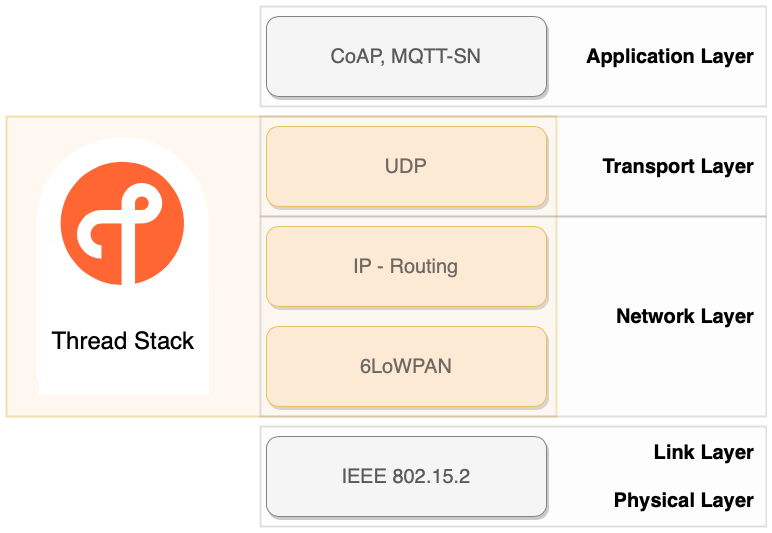
\includegraphics[width=0.6\textwidth]{Overview Thread.png}
	\caption{Übersicht Thread Protokoll}\label{fig:ÜbersichtThreadProtokoll}
\end{figure}

\subsection{Application Layer}\label{subsec:CoAP}
Da das Thread Protokoll auf einer UDP Kommunikation basiert, ist die Wahl des Applikation Layers, dem Entwickler freigestellt. Grundsätzlich ist jedes Protokoll einsetzbar, dass auf einer UDP-Kommunikation basiert. Da Thread das Netzwerkmanagement über das Constrained Application Protocol (CoAP) abfertigt, wird CoAP in diesem Kapitel etwas näher erläutert.

\subsubsection{CoAP}\label{subsubsec:CoAP}
Das Constrained Application Protocol (CoAP) ist ein spezialisiertes Web-Übertragungsprotokoll das dafür entwickelt wurde, um eingeschränkten Geräten die Teilnahme am IoT zu ermöglichen. CoAP ist durch seinen niedrigen Stromverbrauch und geringen Netzwerk-Overhead dafür ausgelegt bei einem Netzwerk mit kleiner Bandbreite und hoher Auslastung zu funktionieren.  UDP wird als grundlegendes Netzwerkprotokoll verwendet, das bedeutet das CoAP ein Client-Server-IoT Protokoll ist, welches die gleichen Methoden wie HTTP verwendet. Das Protokoll wird für Machine-to-Machine (M2M)-Anwendungen wie intelligente Energie- und Gebäudeautomatisierung verwendet. Dank diesen Eigenschaften ist es möglich CoAP bei Stromsparenden Modulen einzusetzen, während TCP-basierte Protokolle nicht in der Lage sind Informationen auszutauschen. Das Protokoll wurde von der Internet Engineering Task Force (IETF) entworfen, CoAP ist in IETF RFC 75852 spezifiziert. In der Tabelle \ref{table:FeaturesCoAP} sind einige Features aufgelistet. \cite{shelby_constrained_2014}

\begin{table}[H]
	\centering
	\begin{adjustbox}{width=1\textwidth}
		\begin{tabular}{@{}|l|l|l|@{}}
			\toprule
			\multicolumn{3}{|c|}{\textbf{Features}}                                                             \\ \midrule
			Web-Protokoll M2M                & Geringer Overhead               & Proxy- und Caching Fähigkeiten \\ \midrule
			Asynchroner Nachrichtenaustausch & URI Uniform Resource Identifier & User Datagram  Protocol  (UDP) \\ \bottomrule
		\end{tabular}
	\end{adjustbox}
	\caption{Features CoAP}
	\label{table:FeaturesCoAP}
\end{table}
\newpage


\subsection{Thread Protokoll Stack}\label{subsec:ThreadProtokollStack}
Der Thread Stack besteht im Grunde aus den beiden Transport und Network Layer (Abbildung \ref{fig:ÜbersichtThreadProtokoll}). Dank dieser Schicht ist es möglich eine geroutete IPv6-Verbindung mit verschiedenen IoT fähigen Geräten aufzubauen. Nachfolgend wird erläutert, wie der Stack aufgebaut ist.

\subsubsection{UDP}\label{subsubsec:UDP}
Das Thread Protokoll schreibt vor, dass ein User Datagram Protocol (UDP) nach dem Standard \cite{postel_user_1980} implementiert werden muss. UDP ist ein minimales und verbindungsloses Netzwerkprotokoll, das ein Versand von Datagrammen innerhalb IP-basierten Netzwerken ermöglicht. Das Protokoll verwendet Ports um die Nachrichten an die richtigen Empfänger zu versenden. Zusätzlich besteht die Möglichkeit eine Prüfsumme mit der Nachricht zu versenden, um Fehlerhafte Nachrichten zu identifizieren. \cite[Seite 6-2]{thread_group_inc_thread_2017}

\subsubsection{IP Routing}\label{subsubsec:IPRouting}
Das Thread Routing-Protokoll ist ein einfaches Distanz-Vektor-Routing-Protokoll. Das Ziel ist es die Routing-Information, die mit einer Nachricht versendet werden kann, zu erhöhen. Aus diesem Grund ist die Anzahl Router im Netzwerk limitiert. Alle Router versenden periodisch ihre Link-Kosten und die Verbindungsqualitäten zu direkt erreichbaren Routern im ganzen Netz. Die endgültigen Routing-Kosten zu einem Ziel, sind demnach die Kosten von allen Routern zum Ziel plus die Kosten zum direkten Nachbarn. Mit dem Trickle-Algorithmus \cite{levis_trickle_2011} wird die Rate festgelegt mit der ein Router seine Informationen ins Netz sendet. \cite[Seite 5-23]{thread_group_inc_thread_2017}

\subsubsection{6LoWPAN}\label{subsubsec:6LoWPAN}
6LoWPAN (IPv6 over Low-Power Wireless Personal Area Networks) ist ein drahtloses Low-Power-Mesh-Netzwerk, bei dem alle Knoten über IPv6-Adressen kommunizieren. Ein Thread Gerät muss das Protokoll implementiert haben. 6LoWPAN dient als Anpassungsschicht zwischen dem MAC Layer und dem Netzwerk Layer. Das Protokoll fragmentiert und setzt die IPv6-Pakete wieder zusammen, damit die grösse der payload vom IEEE 802.15.4 Protokoll übereinstimmt. 6LoWPAN adaptiert somit die IPv6-Pakete auf die IEEE 802.15.4 Pakete, die von der Radioschnittstelle gesendet werden. \cite{thubert_compression_2011} In der Tabelle \ref{table:Features6LoWPAN} sind einige Features aufgelistet. \cite[Seite 3-10]{thread_group_inc_thread_2017}
\begin{table}[H]
	\centering
	\begin{adjustbox}{width=1\textwidth}
		\begin{tabular}{@{}|l|l|l|@{}}
			\toprule
			\multicolumn{3}{|c|}{\textbf{Features}}                                                      \\ \midrule
			Offene IP Standards         & Unterstützt Schlafende Endgeräte & Skalierbares Mesh-Routing   \\ \midrule
			End-Zu-End IP Kommunikation & Selbst Heilendes Netzwerk        & Offener Standard (RFC 6282) \\ \bottomrule
		\end{tabular}
	\end{adjustbox}
	\caption{Features 6LoWPAN}
	\label{table:Features6LoWPAN}
\end{table}

\subsection{Link und Physical Layer}\label{subsec:IEE802154}
Das Thread Protokoll verwendet im Link und Physical Layer das IEEE 802.15.4 Protokoll. \cite{ieee_computer_society_ieee_2020} \cite[Seite 3-2]{thread_group_inc_thread_2017}
\newpage

\subsection{Netzaufbau und Topologie}\label{subsec:NetzaufbauTopologie}
In den nachfolgenden Unterkapiteln wird erklärt, wie das ganze Thread Netzwerk aufgebaut und verwaltet wird.

\subsubsection{Node Rollen}\label{subsubsec:NodeRollen}
Wie im Bild \ref{fig:ThreadDeviceRoles} ersichtlich, wird das Thread Netzwerk in zwei verschiedene Rollen aufgeteilt. \cite[Seite 1-4]{thread_group_inc_thread_2017}

\begin{figure}[H]
	\centering
	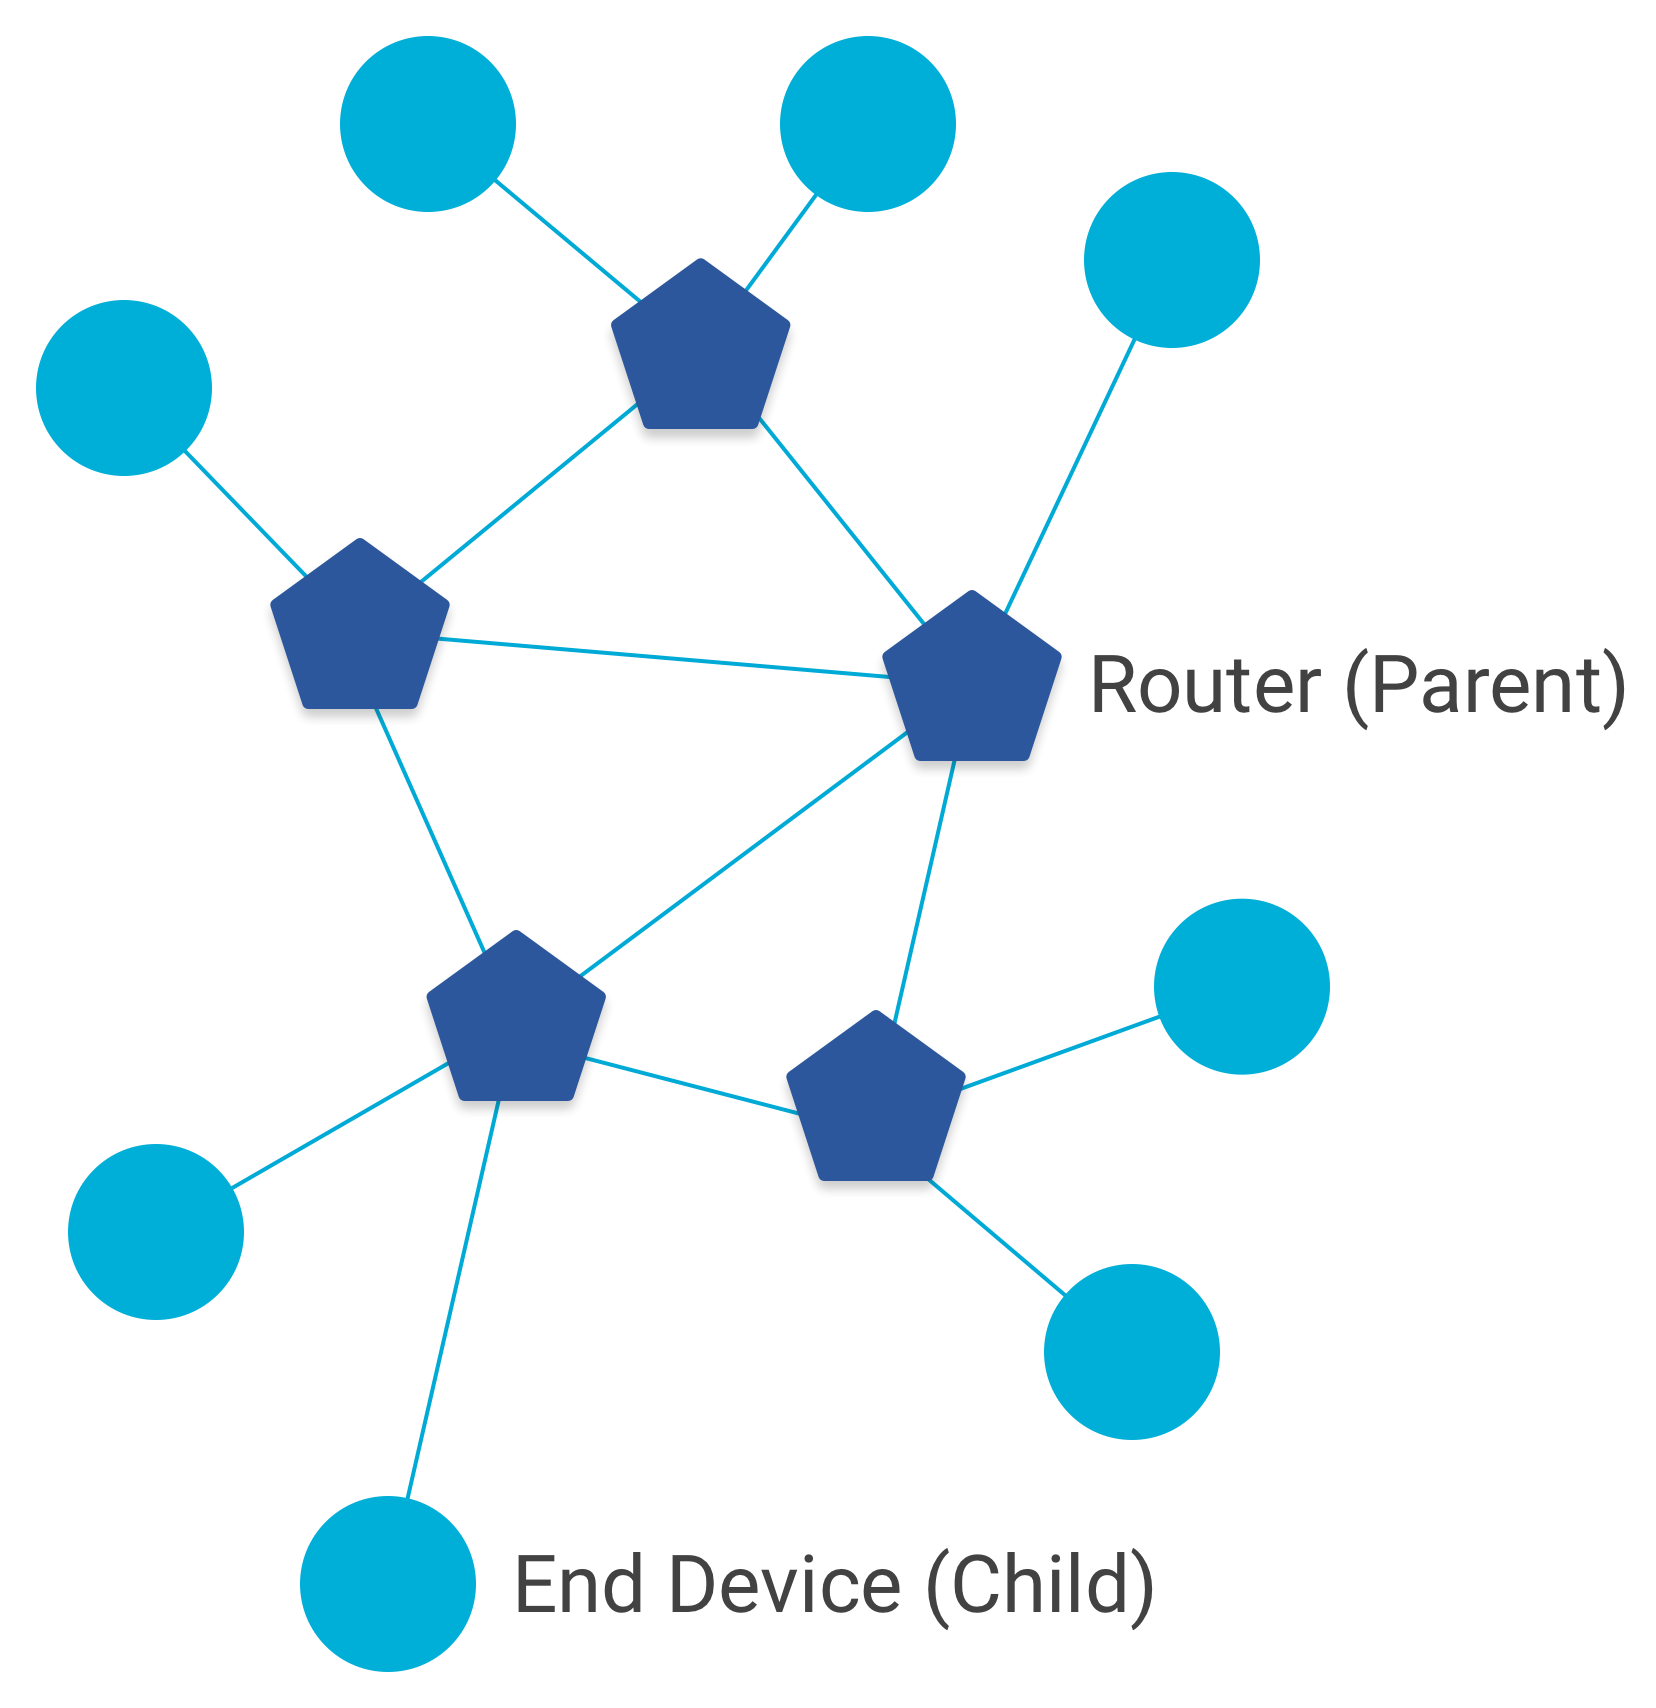
\includegraphics[width=0.6\textwidth]{ot_device_roles.png}
	\caption{Thread Device Roles \cite{openthread_ot-primer-roles_2xpng_2016}}\label{fig:ThreadDeviceRoles}
\end{figure}

\paragraph{Router:}
Ein Gerät mit der Router Rolle leitet alle Pakete für Netzwerkgeräte weiter und hält aus diesem Grund seinen Transceiver jederzeit aktiviert. Weiter bietet der Router sichere Commissioning-Dienste für Geräte an, die versuche dem Netzwerk beizutreten. \cite[Seite 1-4]{thread_group_inc_thread_2017}

\paragraph{Endgerät:}
Ein Gerät mit der Rolle Endgerät kommuniziert hingegen nur mit einem einzelnen Router und kann seinen Transceiver deaktivieren, falls dieser nicht benötigt wird. Das Endgerät kann deshalb seine Leistung reduzieren und trotzdem voll funktionsfähig im Netzwerk kommunizieren. Da der Transceiver sporadisch abgeschaltet wird, leitet das Endgerät keine Pakete für andere Netzwerkgeräte weiter. \cite[Seite 1-4]{thread_group_inc_thread_2017}

\newpage
\subsubsection{Node Typen}\label{subsubsec:NodeTypen}
Ausserdem können die Thread Geräte, wie in Abbildung \ref{fig:ThreadDeviceTypes} zu sehen ist, in zwei verschiedene Node Typen unterteilt werden: \cite[Seite 1-4]{thread_group_inc_thread_2017}
\begin{figure}[H]
	\centering
	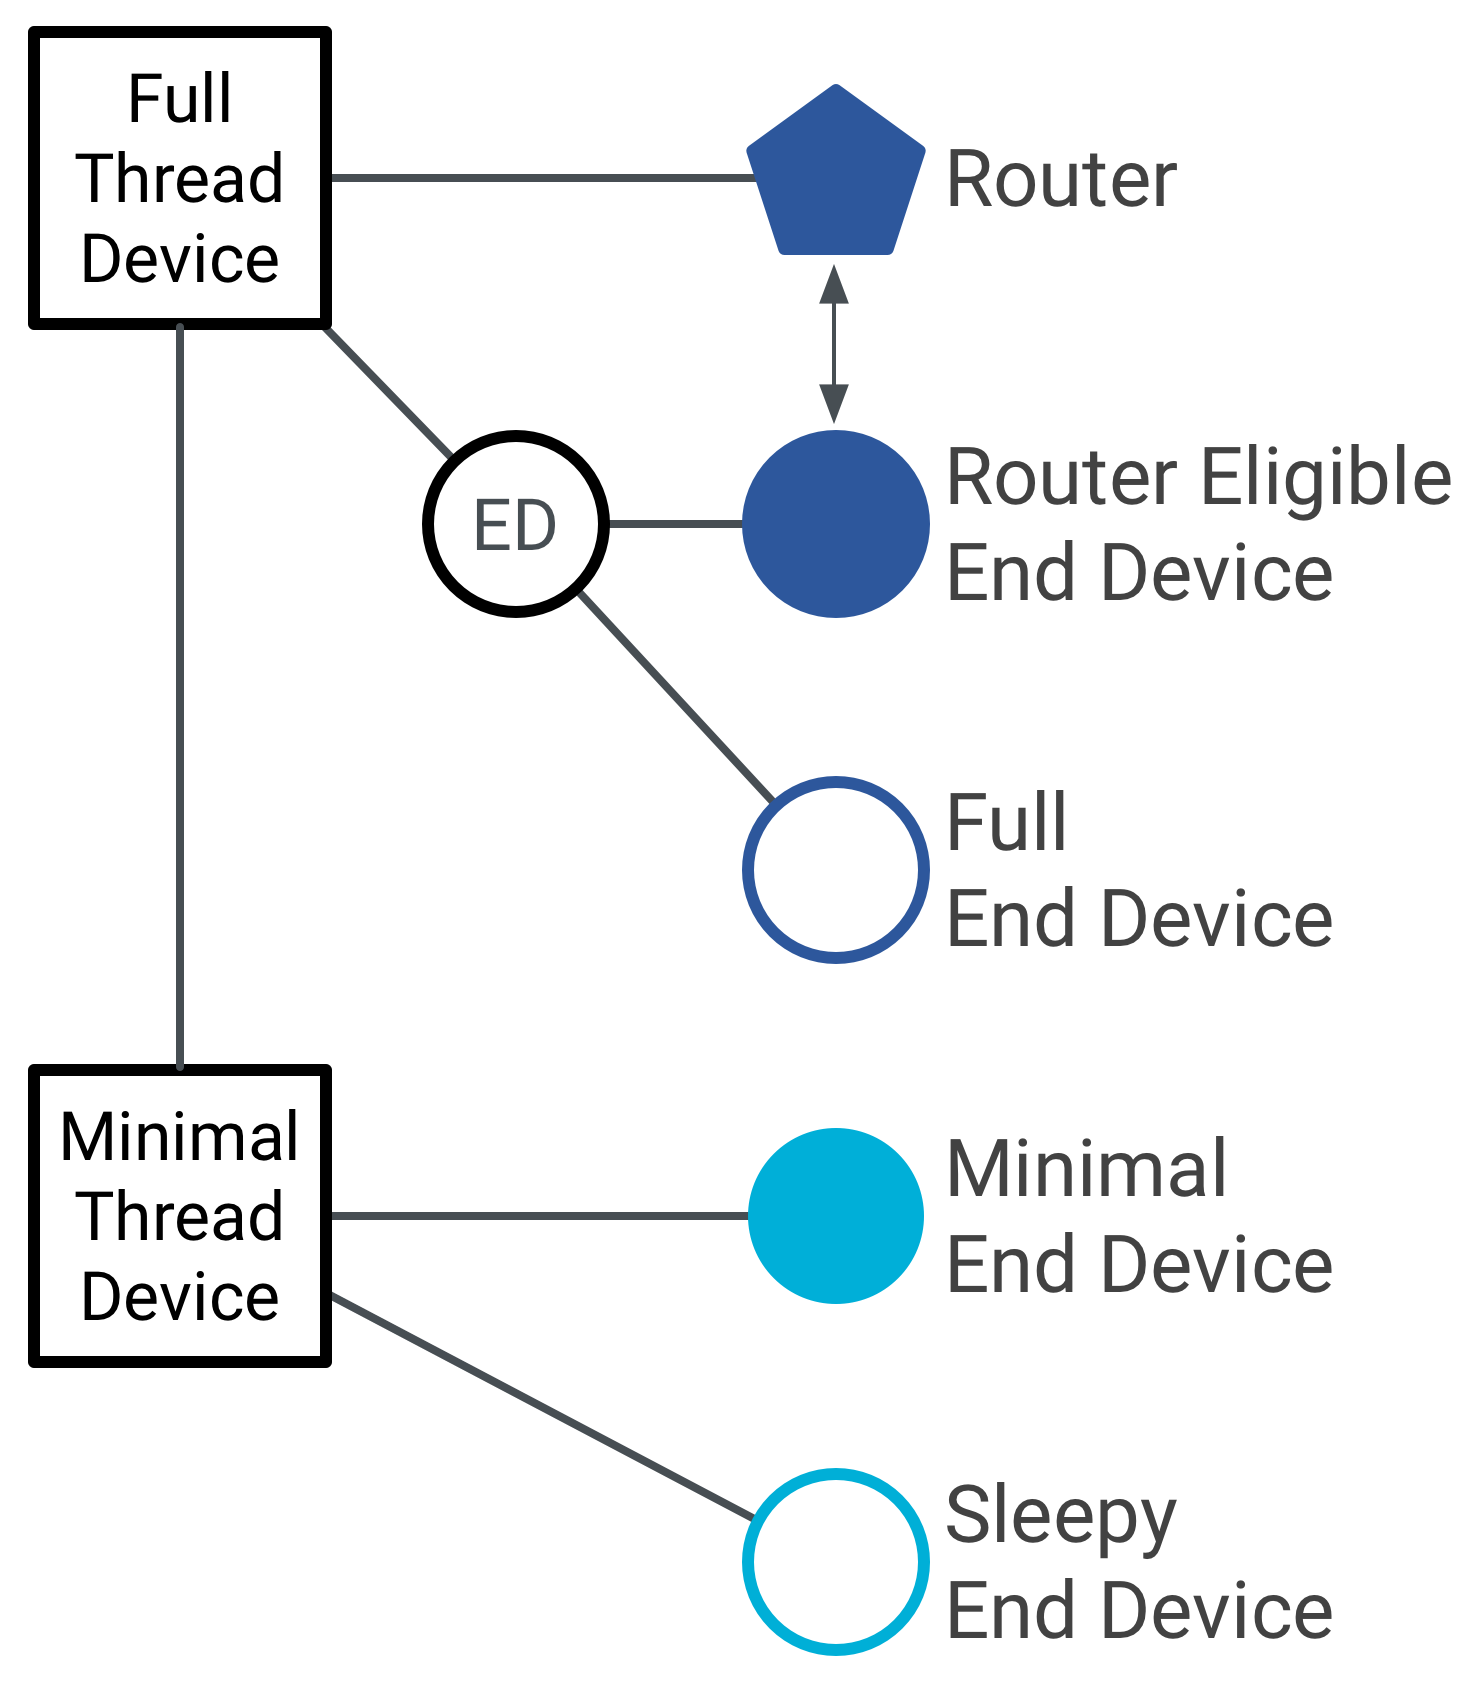
\includegraphics[width=0.39\textwidth]{ot_device_types.png}
	\caption{Thread Device Types \cite{openthread_ot-primer-taxonomy_2xpng_2016}}\label{fig:ThreadDeviceTypes}
\end{figure}

\paragraph{Full Thread Device (FTD):}\label{par:FullThreadDevice}
Ein Full Thread Device (FTD) hat sein on-chip-radio immer aktiviert, erhält und leitet alle Multicast Nachrichten weiter und verwaltet die IPv6-Adresszuordnungen. Ein FTD kann als Router oder als Endgerät arbeiten. Es gibt drei Arten von FTDs: \cite[Seite 1-4]{thread_group_inc_thread_2017}

\begin{itemize}
	\item \textbf{Router}
	\item \textbf{Router Eligible End Device (REED)} - Kann Router oder Endgerät sein.
	\item \textbf{Full End Device (FED)} - Kann nur ein Endgerät sein.
\end{itemize}


\paragraph{Minimal Thread Device (MTD):}
Ein Minimal THread Device leitet keine Multicast Nachrichten weiter, das Gerät kommuniziert nur über einen Router mit dem Netzwerk. Ein MTD kann nur als Endgerät arbeiten. \cite[Seite 1-4]{thread_group_inc_thread_2017}

\begin{itemize}
	\item \textbf{Minimal End Device (MED)} - Transceiver ist immer eingeschaltet und muss keine Nachrichten vom Router abfragen. 
	\item \textbf{Sleepy End Device (SED)} - Transceiver ist ausgeschaltet, wacht nur auf um Nachrichten vom Router abzufragen.
\end{itemize}

\paragraph{Leader:}
Der Thread Leader ist ein Router, der für die Verwaltung aller Router im Netzwerk verantwortlich ist. Der Leader wird dynamisch selbst vom Netzwerk gewählt und hat Zugriff auf das gesamte Thread Netzwerk. Er verteilt auf ganzer Netzwerksebene Konfigurationsinformationen. In jedem Netzwerk gibt es immer nur einen Leader. \cite[Seite 1-4]{thread_group_inc_thread_2017}

\paragraph{Boarder Router:}
Ein Border Router ist ein Gerät, das Informationen zwischen dem Thread Netzwerk und einem nicht Thread Netzwerk weiterleitet. Mit dem Border Router ist es möglich das Thread Netzwerk über das Internet zu erreichen. Es besteht zudem die Möglichkeit das Thread Netzwerk über den Border Router zu konfigurieren. So kann z.B. mit einer Bluetooth Verbindung einzelne Knoten hinzugefügt oder entfernt werden. \cite[Seite 1-4]{thread_group_inc_thread_2017}

\subsubsection{IPv6 Adressierung}\label{subsubsec:IPv6Adressierung}
Die Thread Knoten kommunizieren in einem IPv6 Adressraum miteinander. In diesem Kapitel wird dies etwas näher erläutert. \cite[Kapitel 5]{thread_group_inc_thread_2017}
\paragraph{Bereiche:}
Wie in der Abbildung \ref{fig:IPv6Adressräume} ersichtlich, gibt es für eine Unicast Nachricht drei verschiedene Adressräume:

\begin{itemize}
	\item \textbf{Link-Lokal} - Beinhaltet alle Geräte, die direkt (ohne Hop) erreichbar sind.
	\item \textbf{Mesh-Lokal} - Beinhaltet alle Geräte innerhalb des selben Thread Netzwerkes.
	\item \textbf{Global} - Beinhaltet jegliche Geräte, auch solche die über einen Border Router erreichbar sind.
\end{itemize}

\begin{figure}[H]
	\centering
	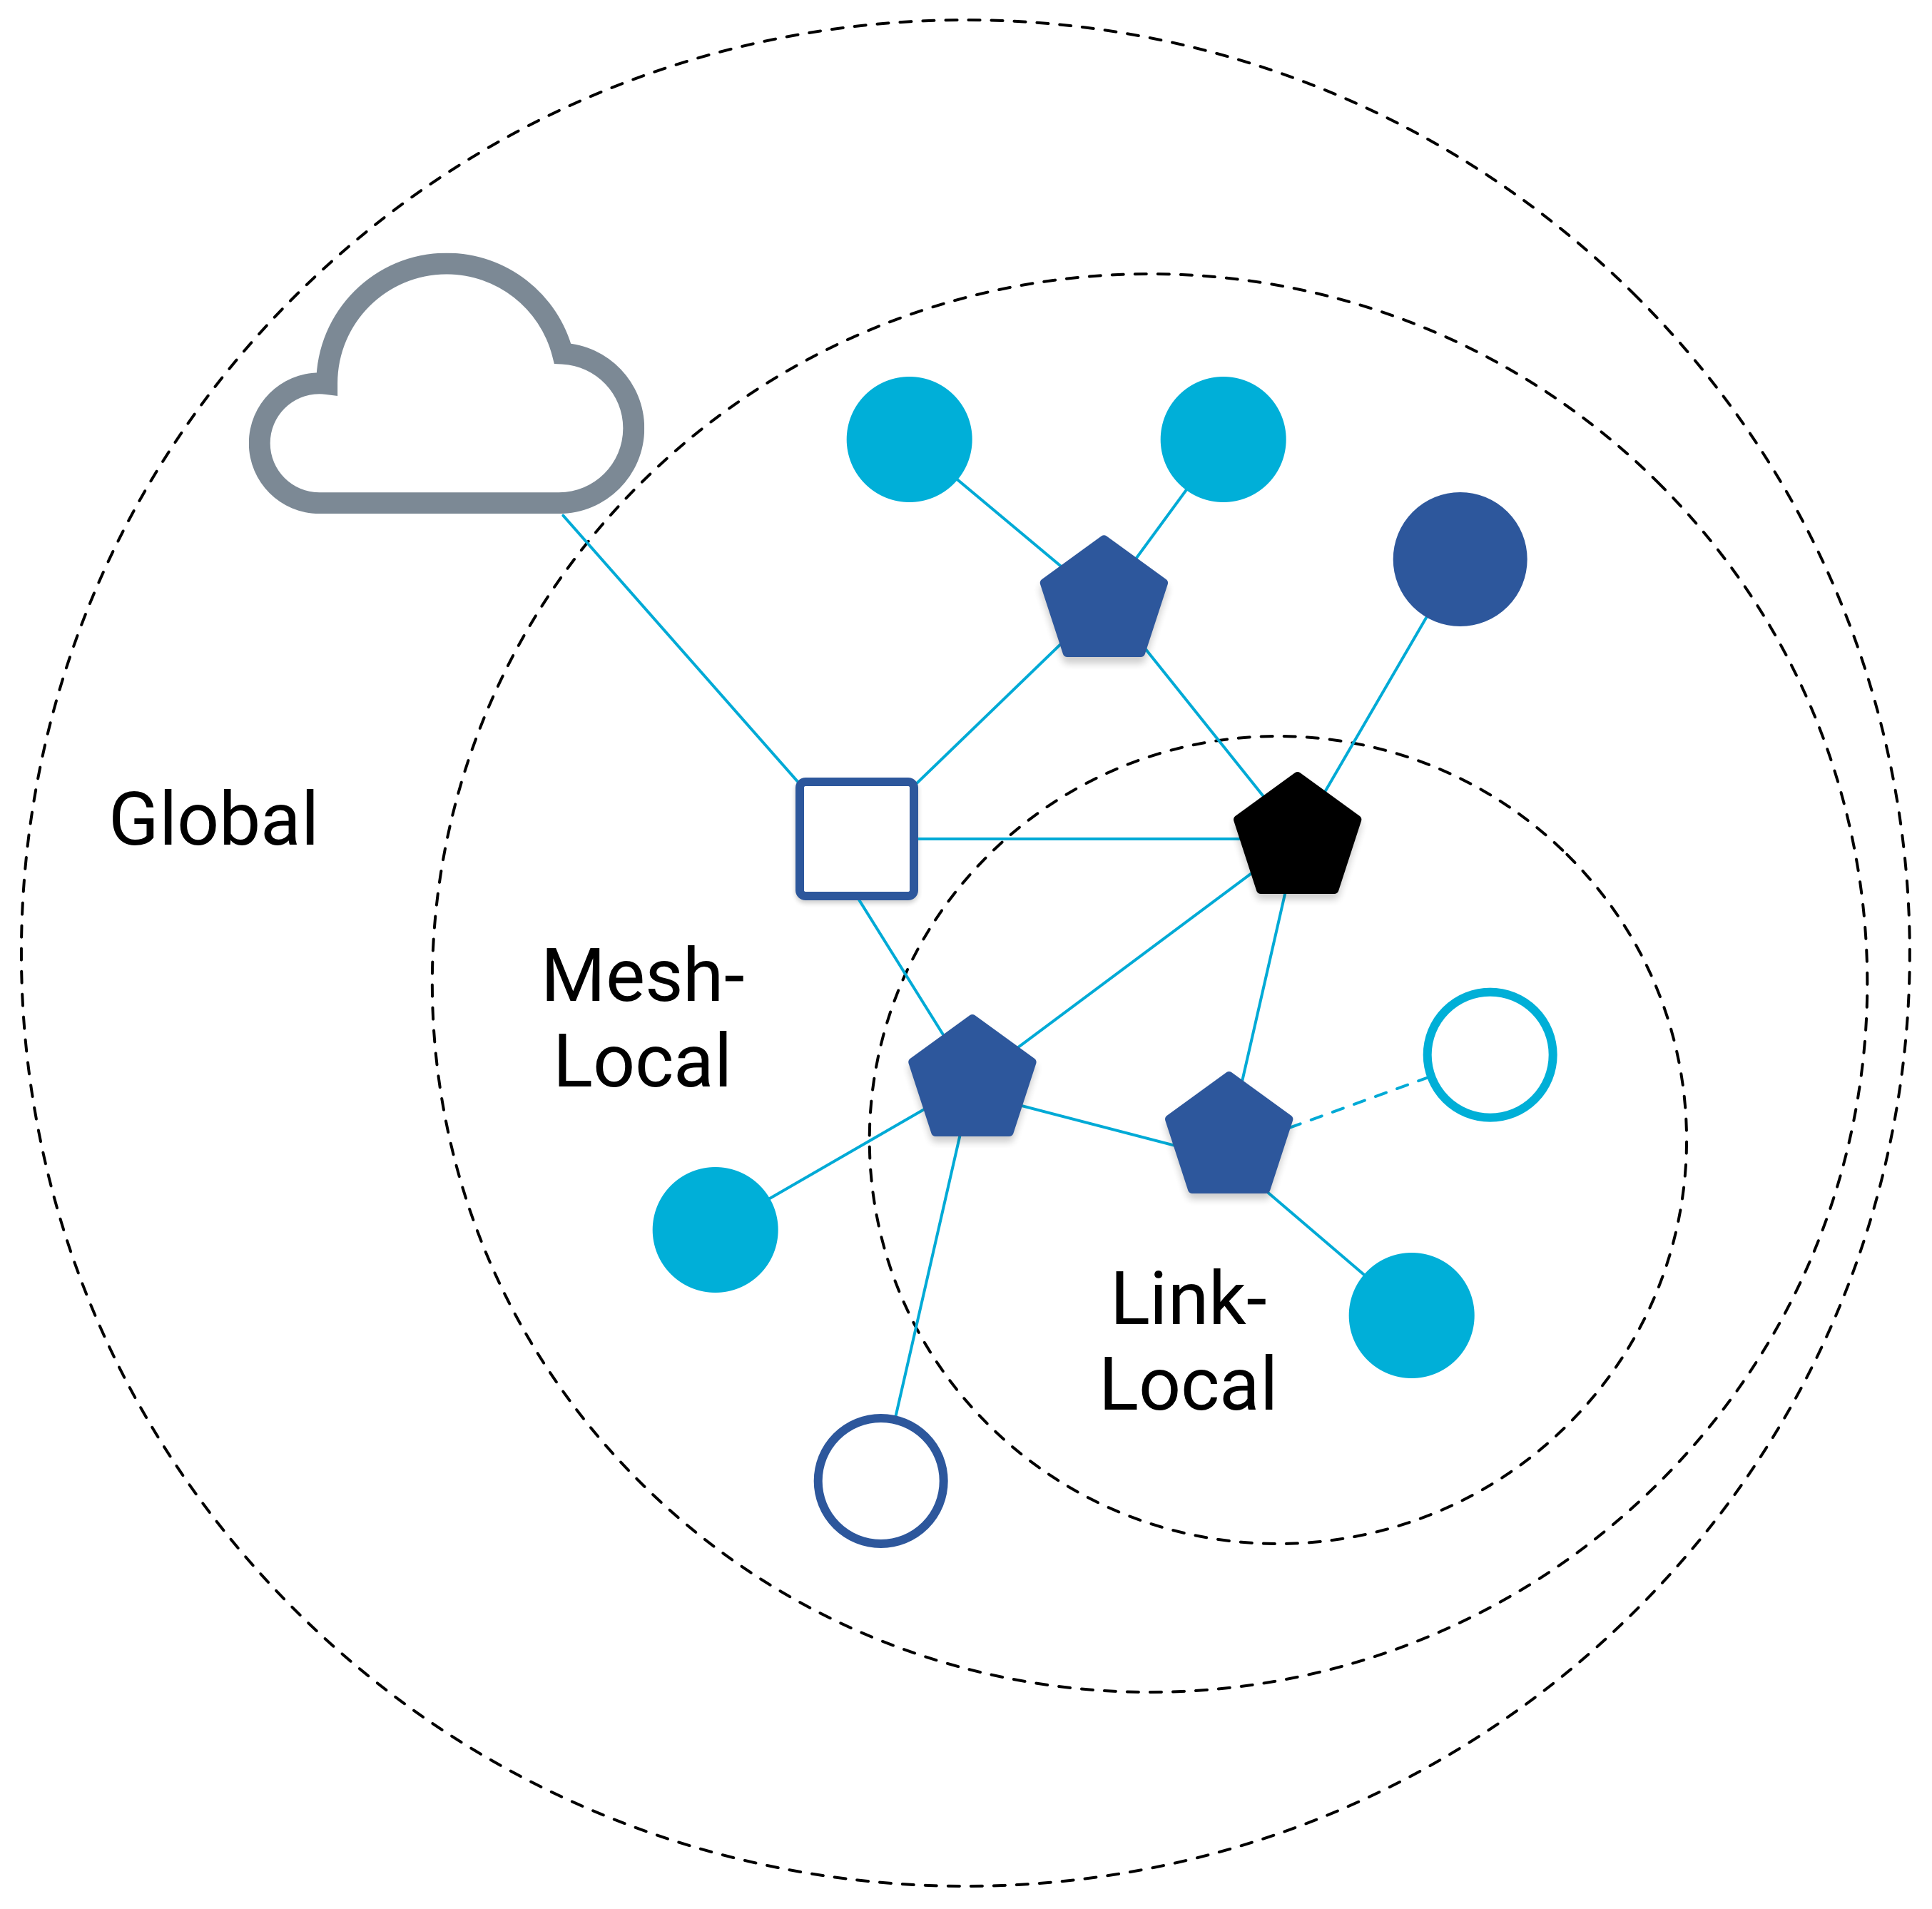
\includegraphics[width=0.5\textwidth]{ot_ip_scopes.png}
	\caption{IPv6 Adressräume \cite{openthread_ot-primer-scopes_2xpng_2016}}\label{fig:IPv6Adressräume}
\end{figure}

\paragraph{Unicast:}
Ein Thread Gerät beinhaltet mehrere IPv6 Adressen, die jede eine andere Funktion hat. Nachfolgend werden alle Adressen kurz aufgelistet: 

\begin{itemize}
	\item \textbf{Link-Lokale Adresse} - Adresse ist nur mit einer einzigen Funkübertragung erreichbar (keine Hops). Diese Adresse wird vom Stack verwendet, um direkt benachbarte Knoten zu finden, um Routing Informationen auszutauschen und die Verbindungen zu konfigurieren. Präfix: fe80::/16
	\item \textbf{Mesh-Lokale EID} - Adresse wird nach dem Eintritt in das Netzwerk zufällig gewählt und ist eindeutig. Mit dieser Adresse sind alle Knoten innerhalb des Thread Netzwerkes erreichbar auch über mehrere Hops. Diese Adresse wird für Anwendungen verwendet. Präfix: fd00::/8
	\item \textbf{Routing Locator} - Diese Adresse lokalisiert die Position des Knoten im Netzwerk. Das bedeutet die Adresse verändert sich, wenn sich die Topologie im Netzwerk ändert. Wird für das Routing verwendet.
	\item \textbf{Anycast Locator} - Wird verwendet, falls der Routing Locator nicht verfügbar ist.
	\item \textbf{Globale Unicast Adresse} - Wird als Globale IPv6 Adresse verwendet für Anwendungen mit Border Router.(Öffentliche IPv6 Adresse) Präfix: 2000::/3
\end{itemize}

\paragraph{Multicast:}
Wenn Nachrichten an mehrere Geräte gleichzeitig gesendet werden müssen, wird eine Multicast IPv6 Adresse verwendet. Die Adressen können unter Einhaltung der zwei Präfixe für Multicast und Unicast, selbst definiert werden. Es gibt jedoch 4 Multicast Adressen, die vordefiniert sind:

\begin{table}[H]
	\centering
	\begin{tabular}{|l|l|l|}
		\hline
		\textbf{IPv6 Adresse} & \textbf{Bereich} & \textbf{Verwendung} \\ \hline
		ff02::1               & Link Lokal       & Alle FTDs und MEDs  \\ \hline
		ff02::2               & Link Lokal       & Alle FTDs           \\ \hline
		ff03::1               & Mesh Lokal       & Alle FTDs und MEDs  \\ \hline
		ff03::2               & Mesh Lokal       & Alle FTDs           \\ \hline
	\end{tabular}
	\caption{Reservierte Multicast Adressen}
	\label{table:ReservierteMulticastAdressen}
\end{table}

\paragraph{Anycast:}
Falls der Routing Lacator nicht verfügbar ist, werden über vordefinierte Anycast Adressen gewisse Funktionen reserviert. In der Tabelle \ref{table:ReservierteAnycastAdressen} sind die Funktionen mit der dazugehörigen reservierten Adresse aufgelistet.

\begin{table}[H]
	\centering
	\begin{tabular}{|l|l|}
		\hline
		\textbf{ALOC16}                                                           & \textbf{Type}            \\ \hline
		0xfc00                                                                    & Leader                   \\ \hline
		0xfc01 - 0xfc0f                                                           & DHCPv6 Agent             \\ \hline
		0xfc10 - 0xfc2f                                                           & Service                  \\ \hline
		0xfc30 - 0xfc37                                                           & Commissioner             \\ \hline
		0xfc40 - 0xfc4e                                                           & Neighbor Discovery Agent \\ \hline
		\begin{tabular}[c]{@{}l@{}}0xfc38 - 0xfc3f\\ 0xfc4f - 0xfcff\end{tabular} & Reserviert               \\ \hline
	\end{tabular}
	\caption{Reservierte Anycast Adressen}
	\label{table:ReservierteAnycastAdressen}
\end{table}

\subsubsection{Netzwerk Aufbau}\label{subsubsec:NetzwerkAufbau}
Das Thread Netzwerk wird mit drei verschiedenen einzigartigen Identifikatoren definiert \cite[Seite 8-18]{thread_group_inc_thread_2017}:

\begin{itemize}
	\item 2-byte Personal Area Network ID. (PAN ID)
	\item 8-byte Extended Personal Area Network ID (XPAN ID)
	\item Netzwerkname
\end{itemize}

Wenn ein Thread Knoten hochfährt und einem Netz aufgenommen werden will oder ein neues Netz kreieren will, scannt das Gerät aktiv nach einem IEEE 802.15.4 Netzwerk in Reichweite:

\begin{enumerate}
	\item Das Gerät sendet einen 802.15.4 Beacon Anfrage von einem spezifischen Channel aus.
	\item Im Gegenzug senden alle Router oder Router fähigen Endgeräte in Reichweite ihre PAN-ID, XPAN-ID und den Netzwerknamen in einem Beacon zurück.
	\item Schritt 1. und 2. werden für alle Channels wiederholt.
\end{enumerate}

Wenn der Knoten alle Netze in Reichweite gefunden hat, kann sich das Gerät entweder einem existierenden Netz verbinden oder eröffnet ein neues Netz.

\newpage

\subsection{Sicherheit}\label{subsec:Sicherheit}
Das Thread Netzwerk wurde so entwickelt, dass während dem Hinzufügen von neuen Geräten und während dem Betrieb ein hohes Mass an Sicherheit gewährleistet ist. Wenn sich ein neues Gerät dem Netzwerk anschliessen möchte, muss dieses mit einem Schlüssel-Vereinbarungs-Mechanismus authentifiziert und autorisiert werden. Sobald das Gerät im Netz aufgenommen wurde, wird jegliche Kommunikation mit einem Netzwerkschlüssel gesichert.

\paragraph{Authentifizierung}
Zur Authentifizierung eines neuen Gerätes, dass dem Netzwerk beitreten möchte wird Grundlegend ein J-Pake(Juggling Password Authenticated Key Exchange) mit elliptischer Kurve verwendet. Mit einem Diffie-Hellmann Schlüsselaustausch, dass eine Elliptische Kurve für die Berechnung verwendet wird ein Schlüssel mit dem Netz und dem Gerät, das dem Netzwerk beitreten möchte festgelegt. Mit dieser Methode wird das Gerät Authentifiziert und erhält die nötigen Schlüssel um dem Netz hinzugefügt zu werden. \cite[Seite 1-4]{thread_group_inc_thread_2017}

\paragraph{Netzwerk Schlüssel}
Das Thread-Netzwerk wird mit einem netzwerkweiten Schlüssel geschützt. Von diesem Schlüssel werden weitere Schlüssel abgeleitet, um den MAC-Layer mit den IEEE 802.15.4 Nachrichten zu schützen. Dadurch wird das Netzwerk vom Abhören und Unterbrechen von Aussenstehenden geschüzt.\cite[Seite 1-5]{thread_group_inc_thread_2017}

\subsection{Thread Software Development Kit}\label{subsec:ThreadSoftwareDevelopmentKit}
In dieser Arbeit wird OpenThread verwendet. OpenThread ist eine open-sorce Implementation von Thread, die von Google umgesetzt und weiterentwickelt wird. Das Software Development Kit von Nordic Semiconductors beinhaltet eine Vorkompilierte Bibliothek des Openthread Stacks. Zuzüglich der Thread Bibliothek befinden sich auch die Normale SDK von Nordic Semiconudtor in dem Kit. Alle Module die für den SoC NRF52840 verfügbar sind, sind auch darin enthalten. Dank der guten Dokumentation und Community-Foren, wurde die Firmware auf der Thread SDK von Nordic aufgebaut. 

\paragraph{IDE}
Für die Erstellung der Firmware wurde die IDE Segger Embedded Systems verwendet. Die Firma Nordic Semiconductor empfiehlt mit dem gebrauch der SDK for Thread and ZigBee das arbeiten mit Segger. Da die alle Beispiel Anwendungen und Dokumentationen mit Segger gemacht wurden, war dies die beste Lösung.
